{
    \def\subBoxWidth{38cm}
    \def\subjectBoxWidth{80cm}
    \def\subjectRowHeight{53.5cm}
    \def\topRowHeightLeft{16.5cm}
    \def\topRowHeightRight{22.5cm}
    \def\bottomRowHeightLeft{23.5cm}
    \def\bottomRowHeightRight{17.5cm}
    \node[anchor=north west, boxStyle, text width=\subjectBoxWidth, anchor=north west, minimum height=\subjectRowHeight] (subjects) at ($(cmsBox.south west)+(0,-1.5)$){
    };

    \node[anchor=north,color=white, text width=70cm] at ($(subjects.north)+(0,-.5)$){
          \small
          The Ghent CMS team is involved in several analyses at CMS, which include supersymmetry searches, top quark physics, and searches for heavy neutral leptons.
          Master students are welcome to join in one of our analyses groups where they get the opportunity to explore the large amounts of new data.
          Under the daily supervision of our CMS team, you will acquire the necessary knowledge to identify particles, select the events of interest and to use big data analysis techniques.
          You get the opportunity to gain experience in an international collaboration, and present/discuss results at CERN.
    };
    
    
    
    

    
    
    
    \node[insideBoxStyle, text width=\subBoxWidth, anchor=north east,minimum height=\topRowHeightLeft] (box1) at ($(subjects.north)+(-1,-10)$){
       \hspace{0.5cm}
       \begin{minipage}{35cm}
         \textbf{Search for the flavour-changing neutral Higgs interactions with top quarks at CMS}\\
         Flavour-changing neutral currents (FCNC) are among the rarest processes in the Standard Model (SM). 
         The probe of the FCNC interactions of a top quark with a Higgs boson represents an excellent probe of various beyond the SM theories. 
         The study includes the search for the top quark FCNC decays in the top quark pair production process, 
         as well as the probe of FCNC effects in the single top associated production with a Higgs boson. 
         One of the tasks in this analysis is to develop an event selection criteria to identify the FCNC processes 
         with a potential use of various Machine Learning techniques. 
       \end{minipage}\\
       \hspace{2.5cm}
       \begin{minipage}{15cm}
         \begin{center}
         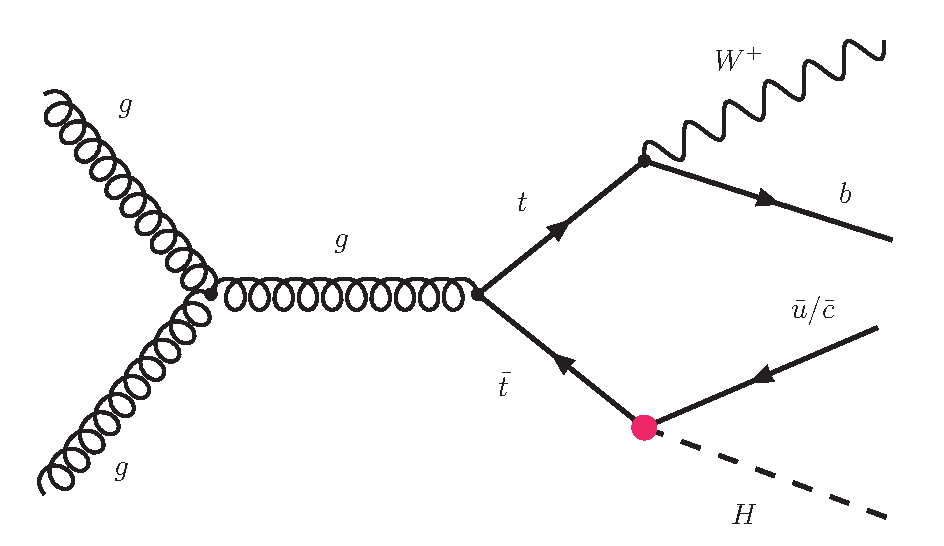
\includegraphics[width=0.9\textwidth]{tH_ttbar_mod.eps} 
         \end{center}
       \end{minipage}
       \hspace{2cm}
       \begin{minipage}{15cm}
         \begin{center}
         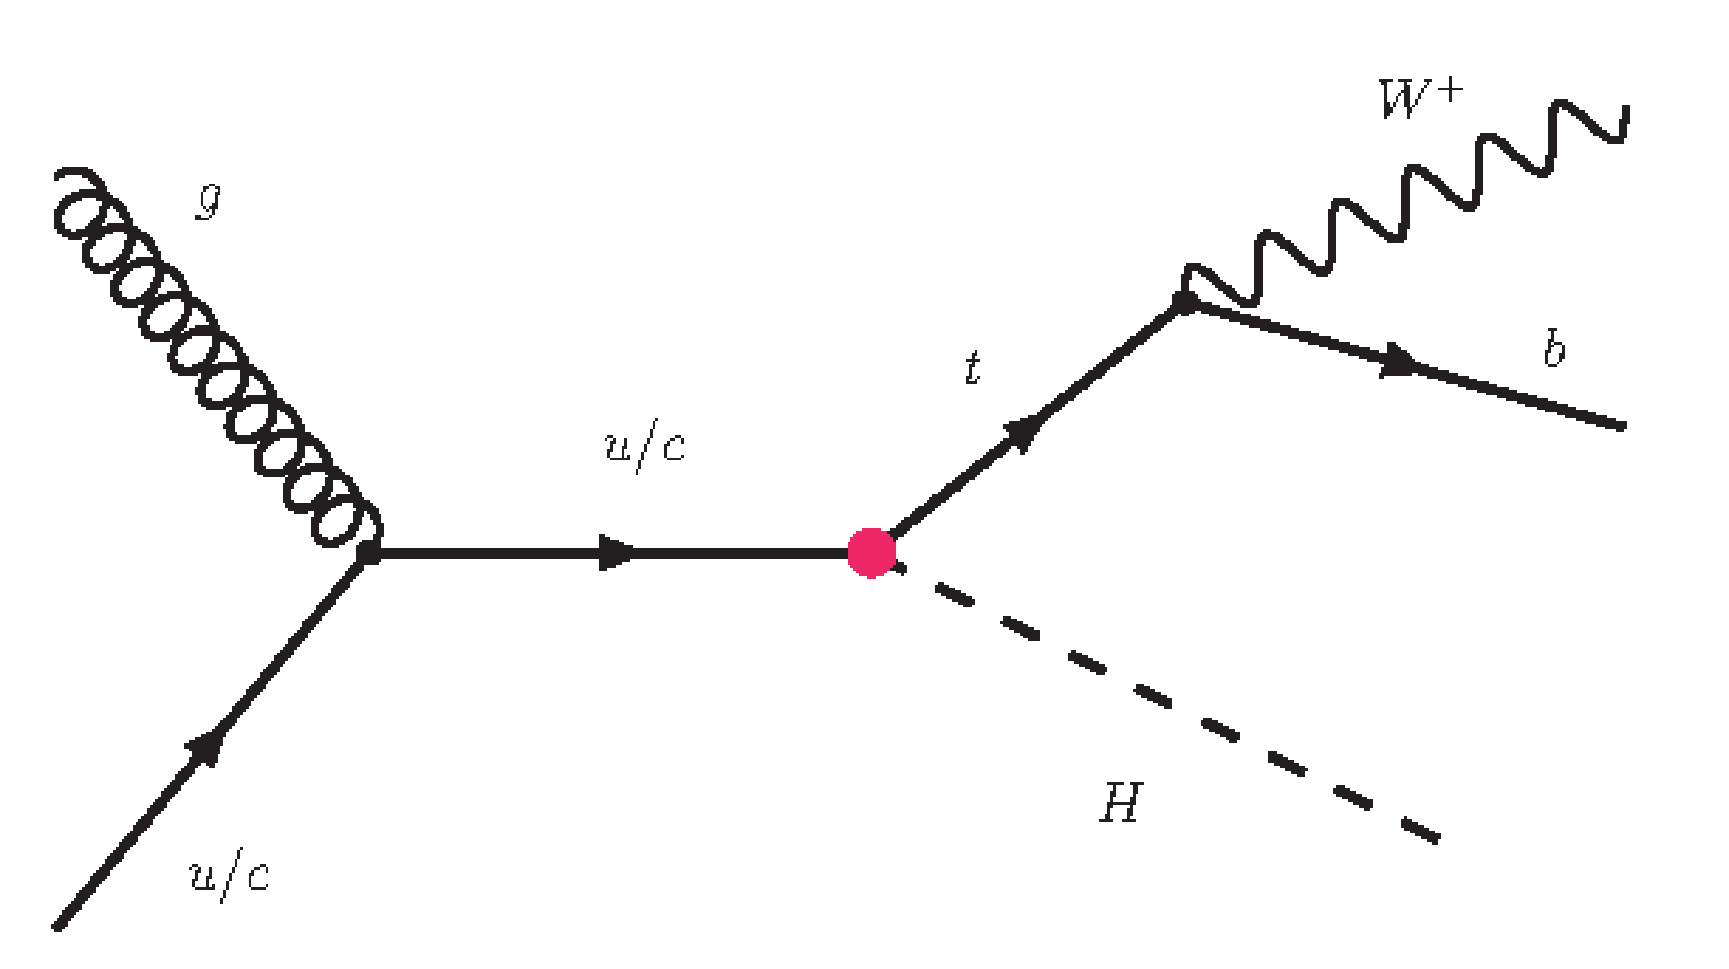
\includegraphics[width=0.9\textwidth]{tH_mod.eps} 
         \end{center}
       \end{minipage}
    };
    \node[insideFancytitle, left=\insideTitleOffset] at ($(box1.north east)+(0,0.5)$){\normalsize Flavour changing neutral currents}; 
   
 

    \node[insideBoxStyle, text width=\subBoxWidth, anchor=north west,minimum height=\bottomRowHeightLeft] (box2) at ($(box1.south west)+(0,-2.5)$){
        \hspace{0.5cm}
        \begin{minipage}{22cm}
          \textbf{A study of displaced tracking efficiency using neutral kaon decays in the CMS detector}\\
          The CMS detector at the CERN LHC was designed for the detection and accurate reconstruction of particles 
          emerging directly from the proton-proton collisions at the detector center. 
          However, some extensions to the standard model of particle physics include undetectable particles that only 
          decay to detectable particles at a relatively large distance from the detector center. 
          The goal of this thesis project is to quantify the efficiency of the CMS detector for this kind of so-called displaced objects, 
          using a partly data-driven technique. The focus will be on the decay of the neutral K-meson to two charged pions. 
          Since the K-meson itself is invisible to the inner part of the detector and has a relatively long lifetime, 
          its decay to two pions yields a similar signature as the exotic `beyond standard model` scenarios one is typically investigating. 
          Using both simulated events and actual data, we will try to measure the efficiency of CMS for measuring displaced decays and 
          estimate the uncertainty on this measurement. 
        \end{minipage}
        \begin{minipage}{13cm}
        \begin{center}
          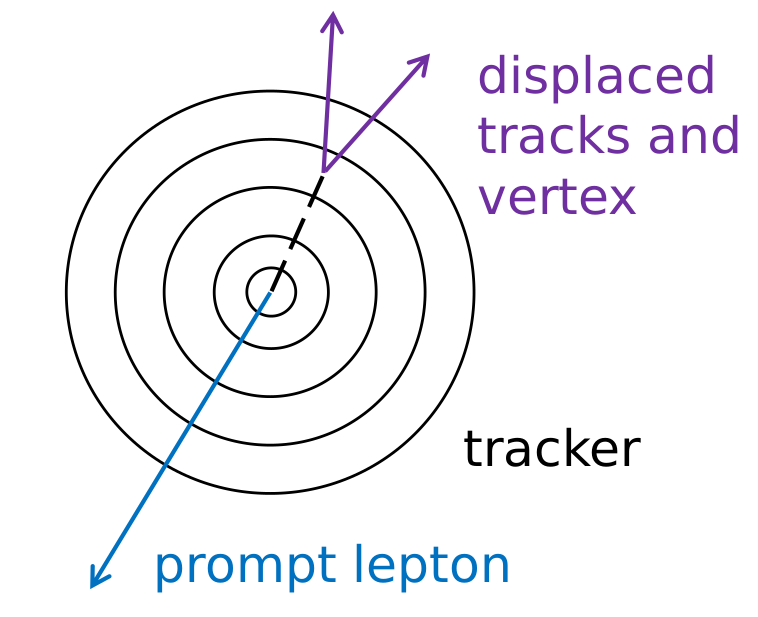
\includegraphics[width=0.9\textwidth]{displacedTracks.png} \\
          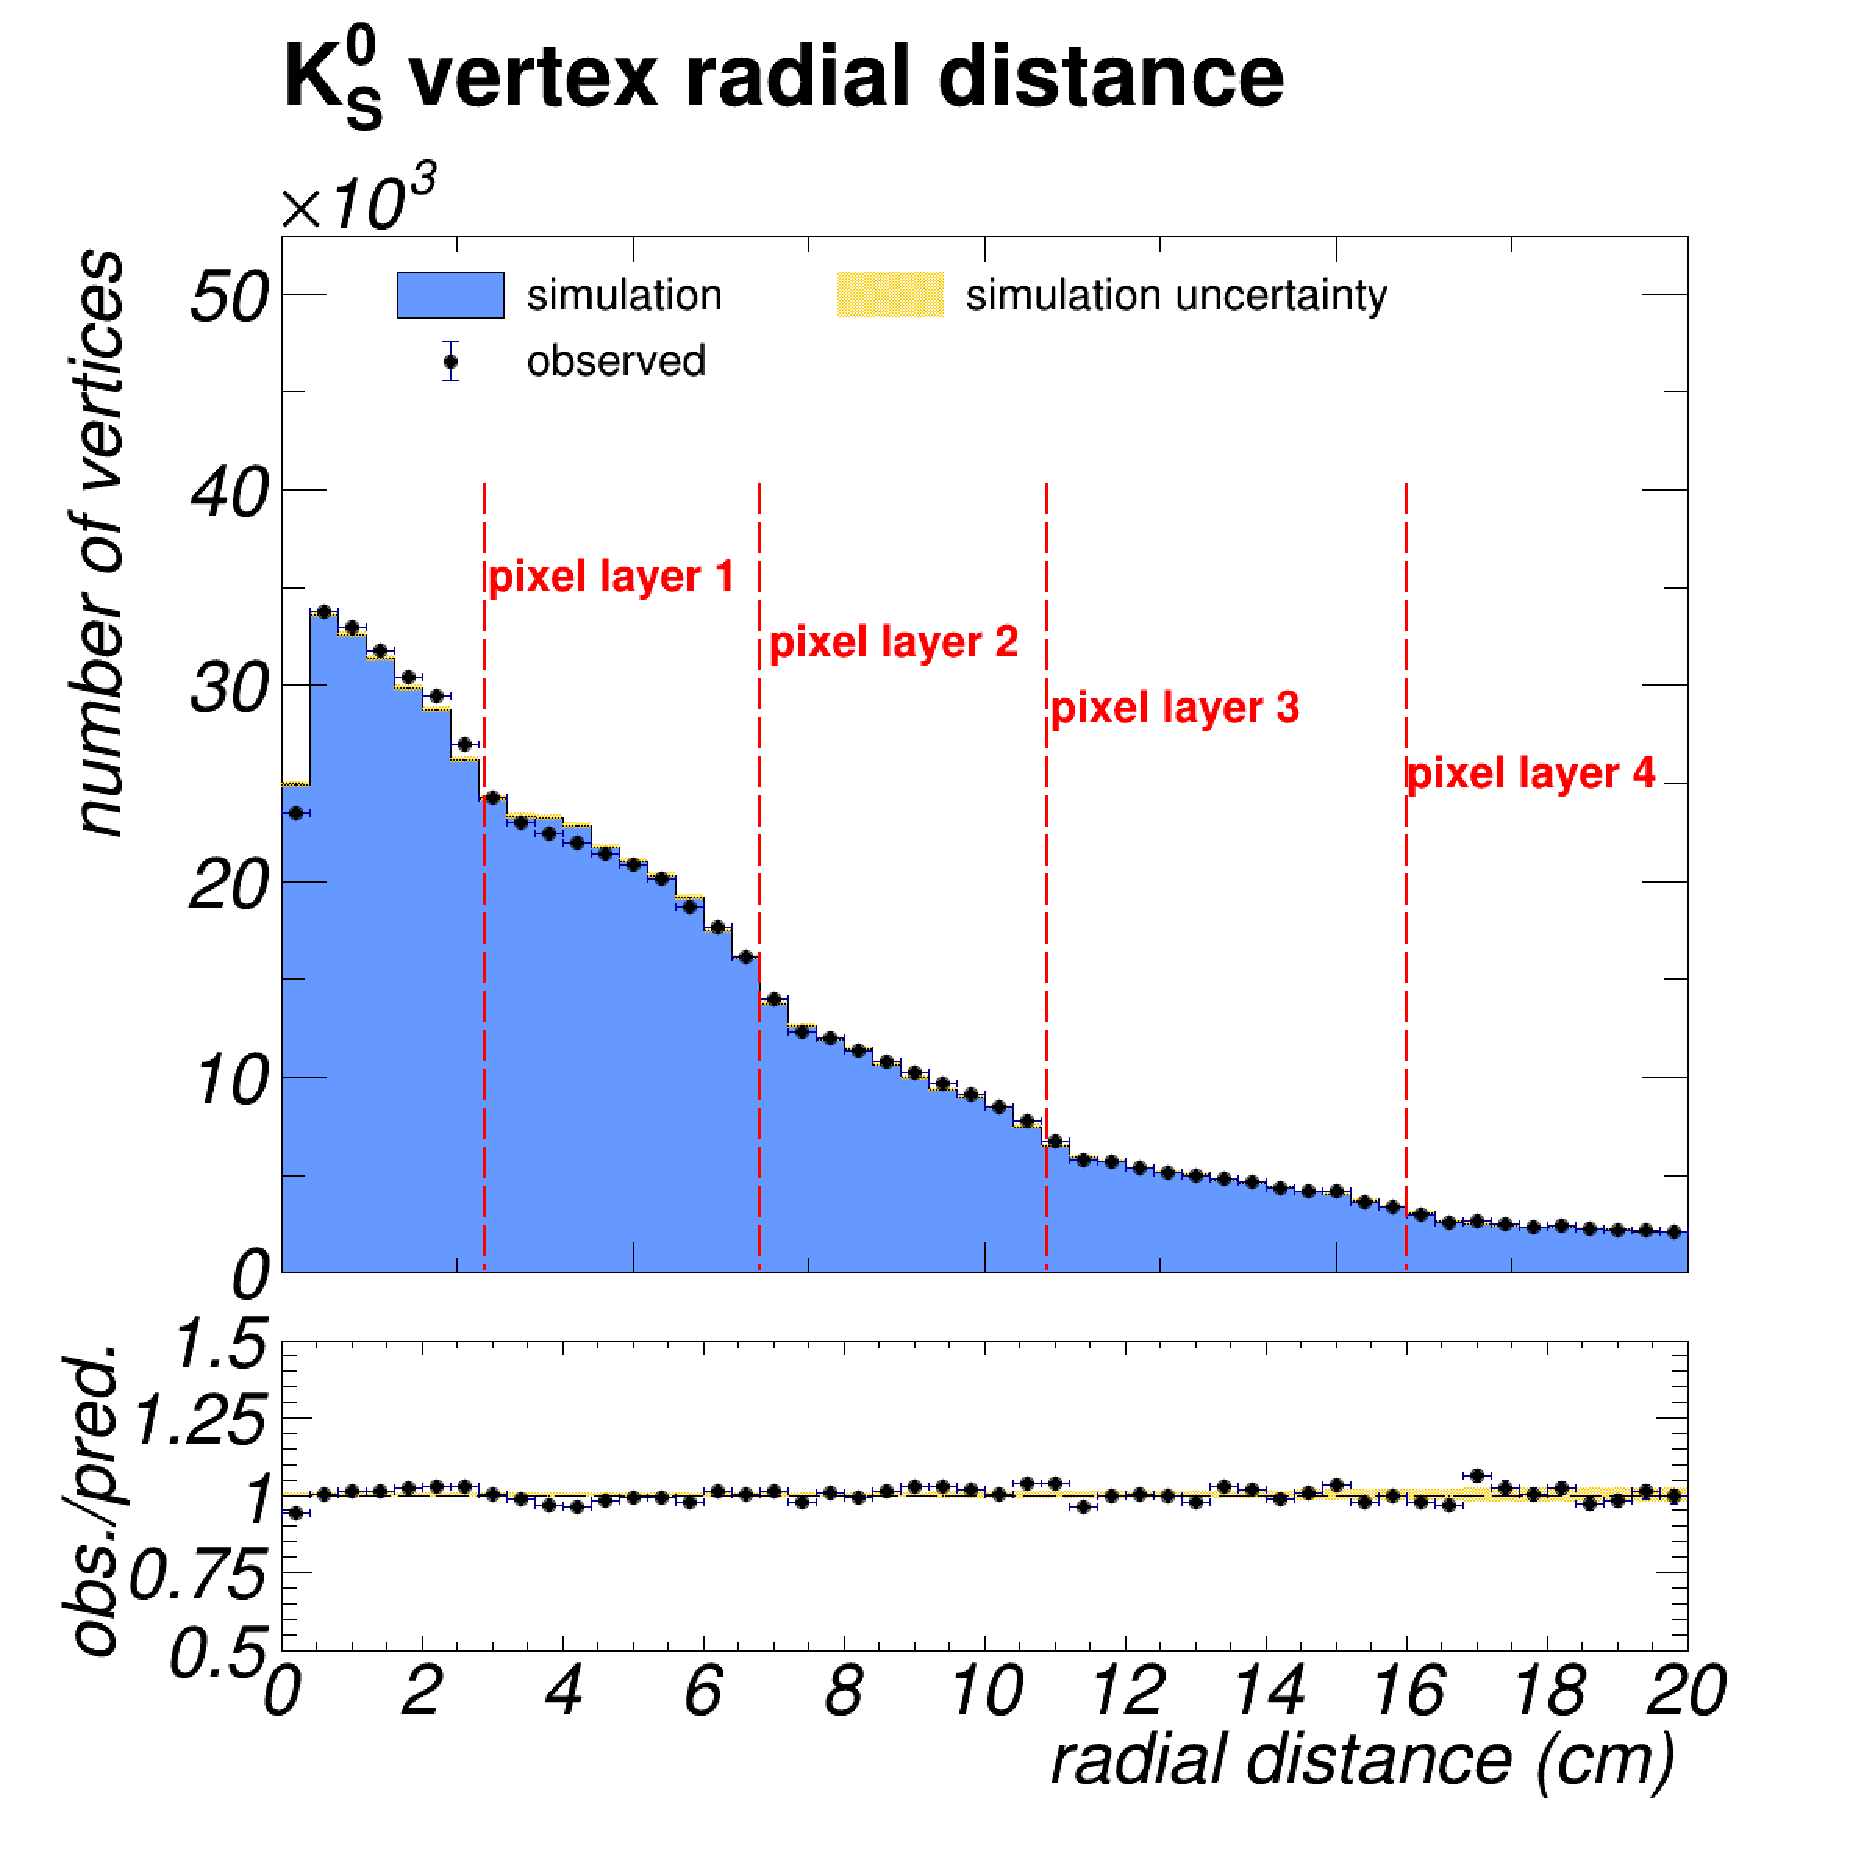
\includegraphics[width=0.9\textwidth]{2017E_detector.pdf} 
        \end{center}
        \end{minipage}

    };
    \node[insideFancytitle, left=\insideTitleOffset] at ($(box2.north east)+(0,0.5)$){\normalsize Tracking};
     
 
 

   
   
    \node[insideBoxStyle, text width=\subBoxWidth, anchor=north west,minimum height=\topRowHeightRight] (box3) at ($(subjects.north)+(1,-10)$){
       \hspace{0.5cm}
       \begin{minipage}{35cm}
         \textbf{Rediscovering the Higgs boson at CMS}\\
         The exact mass generation mechanism still remains to be an open question in particle physics. 
         The study of the Higgs boson production represents the direct probe of the Higgs boson couplings to other fundamental constituents of nature. 
         Any deviations in the measured values of these parameters from the SM predictions would directly point to the new physics phenomena. 
         The study is proposed for the analysis of the CMS detector data to rediscover the Higgs boson in one of its production processes
         by additionally involving Machine Learning techniques to further boost the final sensitivity in the analysis. 
       \end{minipage}
       \begin{center}
         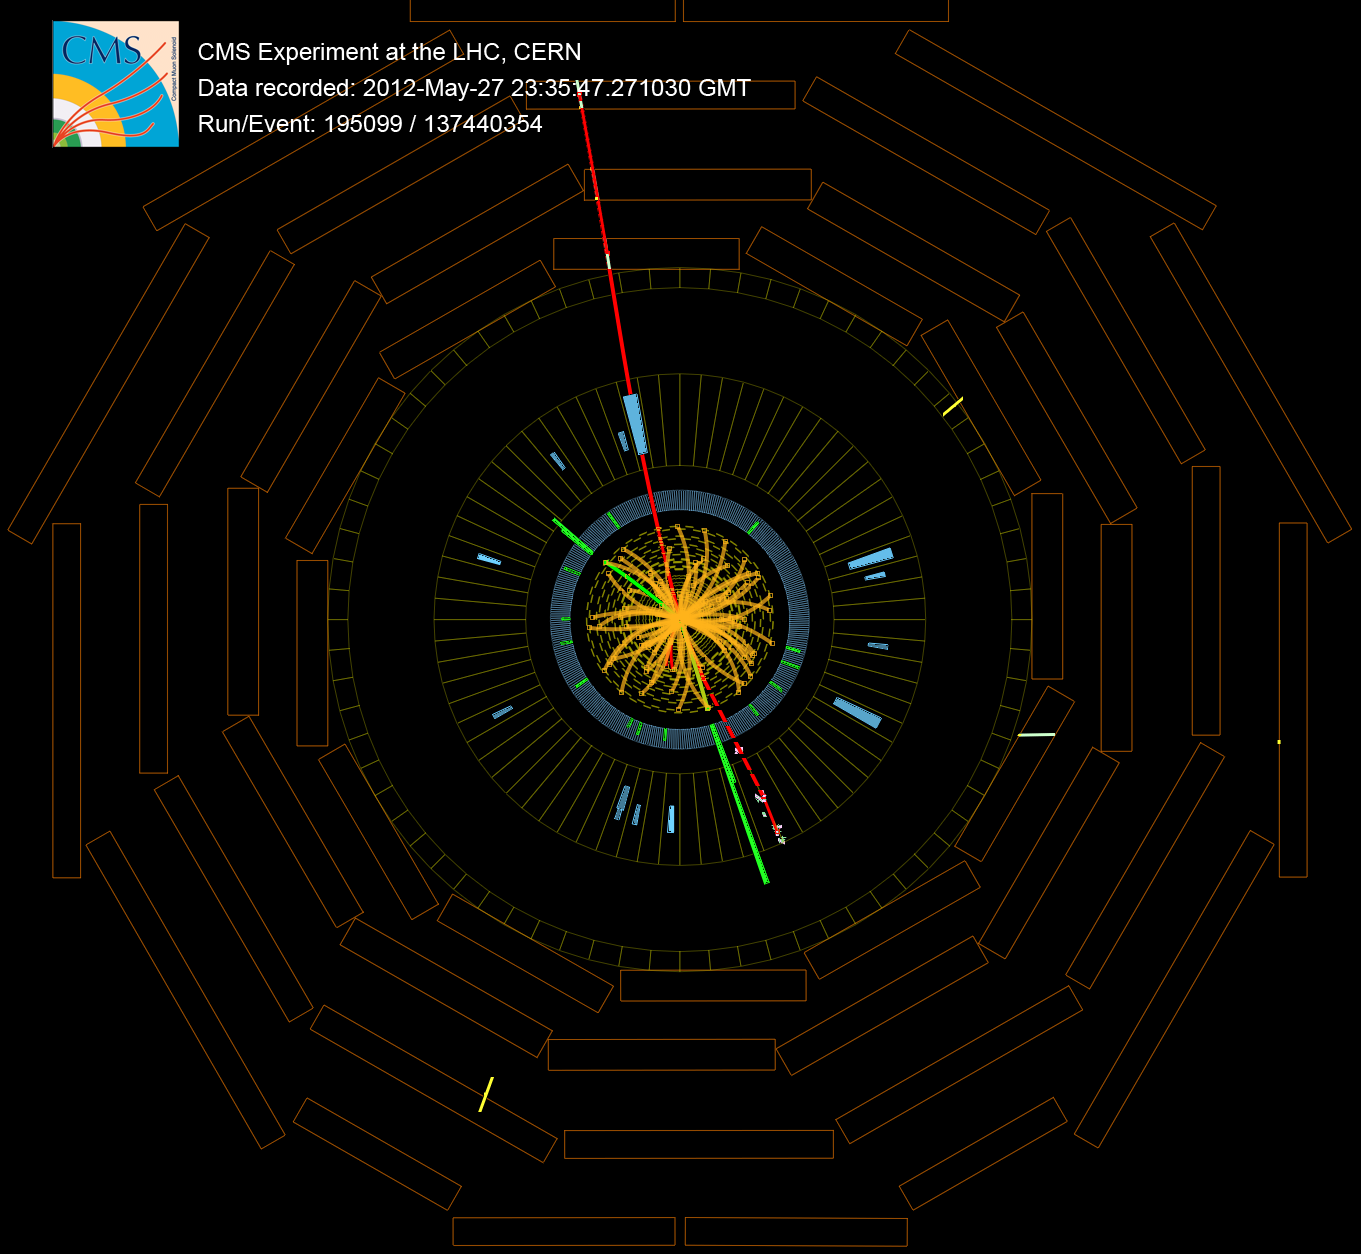
\includegraphics[height=13cm]{higgs.png} 
         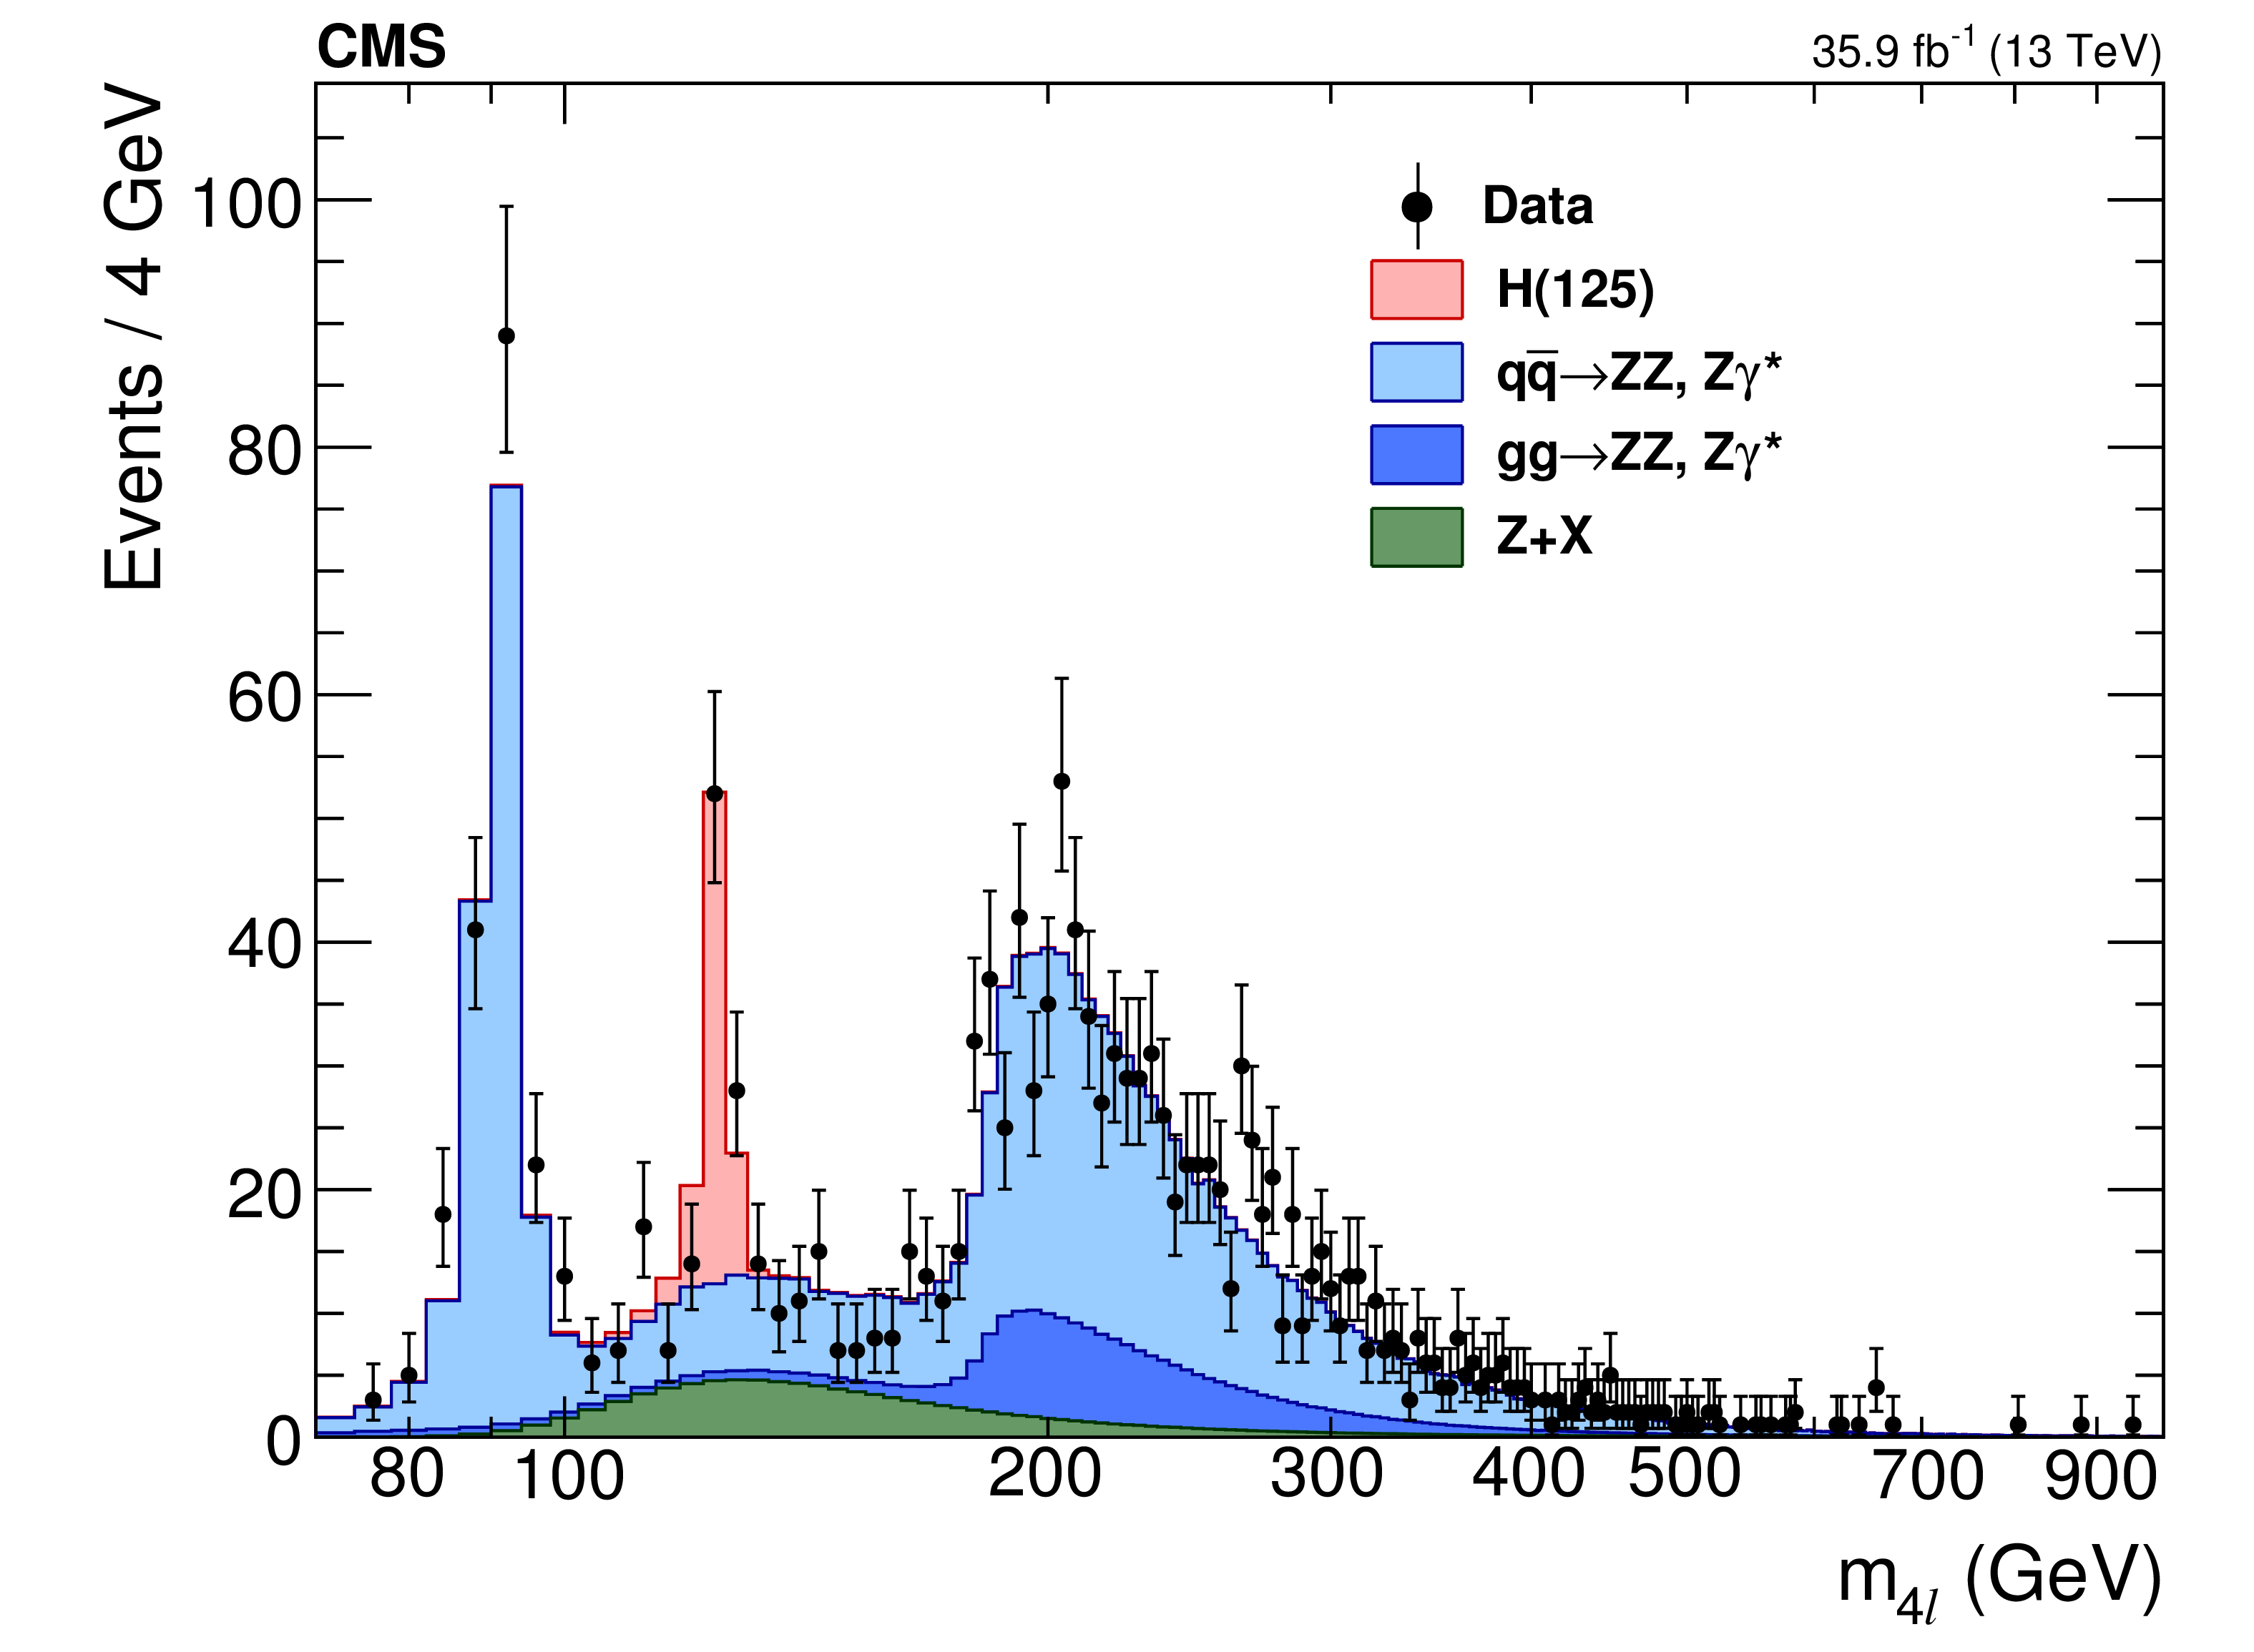
\includegraphics[height=13cm]{higgs2.png} 
       \end{center}
    };
    \node[insideFancytitle, left=\insideTitleOffset] at ($(box3.north east)+(0,0.5)$){\normalsize Rediscovering the Higgs boson at CMS};
    

    \node[insideBoxStyle, text width=\subBoxWidth, anchor=north east,minimum height=\bottomRowHeightRight] (box4) at ($(box3.south east)+(0,-2.5)$){
       \hspace{0.5cm}
       \begin{minipage}{25cm}
         \textbf{Enlightening the top quark: a study of the interaction of a top quark and a photon with the CMS detector}\\
         The distinctive properties of the top quark put it in a special place of the Standard Model (SM).
         A precise study of the strength of the interaction of this particle with other fundamental constituents 
         represents an important test of the SM predictions. The study of the processes with the production 
         of a top quark in association with a photon represents a direct probe of the electroweak charge and interaction couplings of the top quark, 
         as well as provides a handle to search for various new physics effects. 
         The proposed analysis will cover the study of the kinematic properties of the processes with the production of top quark pairs 
         with one or more photons in the final state with the CMS detector. 
         The possible tasks include the study of the photon identification in data, 
         as well as the development of the event selection criteria exploiting the full event reconstruction. 
         A potential gain from the use of Machine Learning techniques will also be explored. 
       \end{minipage}
       \begin{minipage}{9cm}
       \begin{center}
         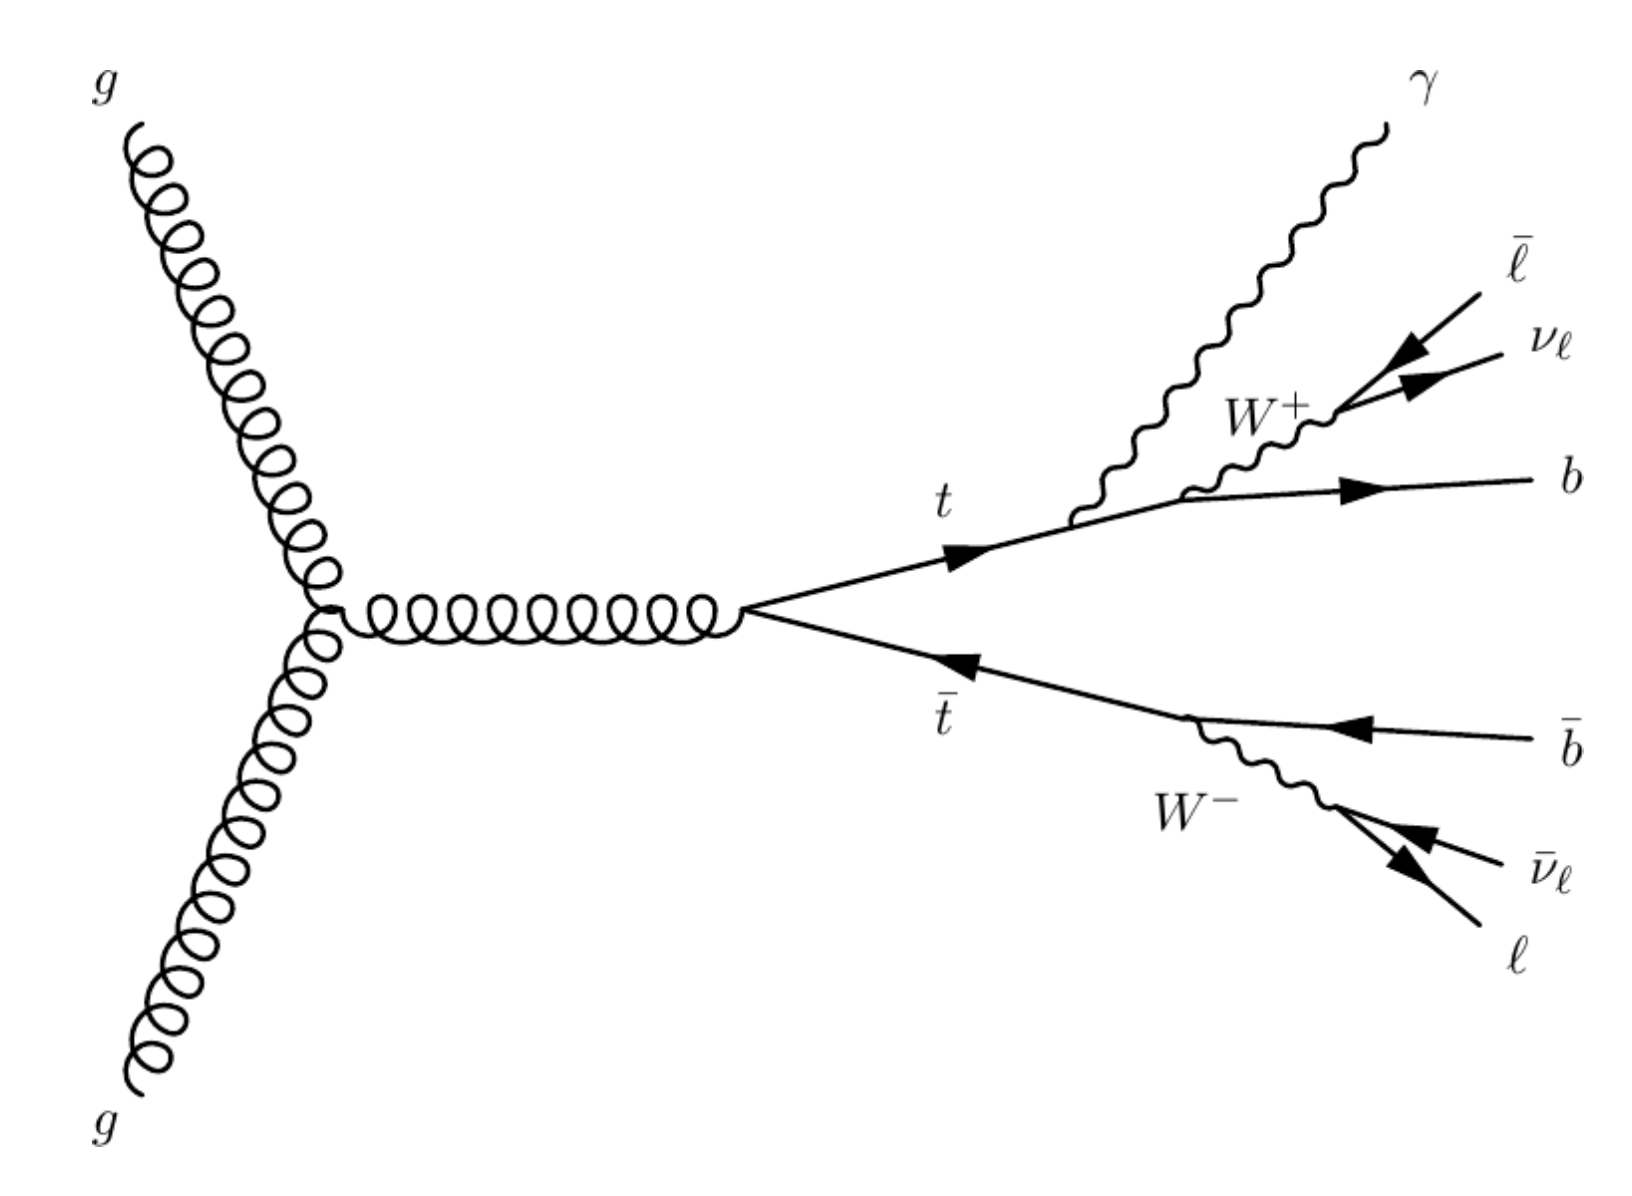
\includegraphics[width=0.9\textwidth]{ttgamma.png} 
       \end{center}
       \end{minipage}
    };
    \node[insideFancytitle, left=\insideTitleOffset] at ($(box4.north east)+(0,0.5)$){\normalsize Interaction of a top quark and a photon}; 
    
    
       
       

}